\documentclass{article}

\usepackage{iclr2027_conference,times}

% Optional math commands from the official ICLR template.
\input{math_commands.tex}

\usepackage{hyperref}
\usepackage{url}
\usepackage{graphicx}下一步建议先处理 .gitignore，把这些垃圾文件隐藏/排除，然后初始化 Git，再开始正式迁移 RewardLens 正文。这样工程会干净很多。
\usepackage{booktabs}
\usepackage{amsmath}
\usepackage{amssymb}

\title{RewardLens: Auditing Visual Evidence Dependence in Multimodal Judges}

% Submission must remain anonymous.
\author{Anonymous Authors}

% DO NOT uncomment for submission.
% \iclrfinalcopy

\begin{document}

\maketitle

\begin{abstract}
Static preference accuracy can fail to distinguish multimodal judges that
behave differently under controlled changes in visual evidence.
% TODO: Replace with frozen RewardLens abstract.
\end{abstract}

\section{Introduction}
\label{sec:introduction}

Multimodal judges compare vision--language outputs and provide preference
signals for model development. They are commonly summarized by static
preference accuracy: given an image, question, and two responses, how often is
the correct response selected? This cross-sectional score does not reveal how
the same decision changes when its visual evidence changes.

This question is adjacent to, but distinct from, controlled perturbation and
failure-to-update studies \citep{lee2026mmjudgebias,park2026mitigating,zhu2026visualflip}.
RewardLens evaluates the residual behavioral variation among judges that an
\emph{independent} static preference evaluation assigns equal or nearly equal
scores. It also tests both a relevant edit, for which the gold preference must
change, and an irrelevant edit, for which it must remain fixed.

We introduce \textbf{RewardLens}, a behavioral audit asking:
\emph{among judges with equal or near-equal measured static accuracy, how much
intervention-behavior variation remains?} An independent natural-image set
measures factor-specific static accuracy. A separate controlled audit then
holds the question and responses fixed while changing the rendered scene. Each
triplet contains a base image, a relevant edit that reverses the gold
preference, and an irrelevant edit that preserves it. Relevant Adaptation (RA)
measures correctness after the relevant edit, conditional on a correct base
decision; Irrelevant Invariance (II) measures the analogous correctness after
the irrelevant edit.

Across eight multimodal judges and four factors---Count, Attribute, Presence,
and Spatial---static similarity can coexist with different measured
intervention behavior. Phi-3.5-Vision and LLaVA-OneVision-7B tie at $80.5\%$
static Attribute accuracy, yet differ in RA by $15.1$ percentage points
(paired-bootstrap 95\% CI: $10.2$--$20.4$ pp). Across all seven within-factor
pairs matched within one static-accuracy point, the descriptive median RA gap
is $15.1$ points, and four gaps are at least $10$ points. Qwen3-VL-4B provides
a concrete transition-level example: on $166/200$ base-correct Count triplets,
the gold preference changes but its prediction does not.

RewardLens does not identify internal reasoning or replace static evaluation.
It shows that a shared measured static score can leave consequential behavioral
variation unresolved. Our contributions are a static-score-matched measurement
framing, a programmatically constructed and validated RewardLens-CLEVR audit
with relevant and irrelevant edits, and an eight-judge evaluation with paired
uncertainty and pre-specified matching-band checks.


\section{Related Work}
\label{sec:related_work}

LLM-as-a-judge research studies the reliability, calibration, and agreement of
automatic preference evaluators, including broad judge benchmarks
\citep{zheng2023judging,tan2025judgebench,zhou2025jetts,yang2025reliablejudge}.
Multimodal judge and reward-model work extends that setting to
image-conditioned outputs and preference data
\citep{chen2024mllmjudge,chen2025mjbench,ko2025flexjudge,yasunaga2025multimodal,
hu2026multimodalrewardbench2,zhang2026r1reward,jin2026omnireward}.
These evaluations primarily characterize performance on fixed examples; they
do not ask whether judges with closely matched scores respond similarly to
controlled changes in visual evidence.

Visual spurious-correlation and counterfactual studies test whether visual
models use task-relevant evidence. MM-JudgeBias and Perceptual Judgment Bias
study controlled perturbations in multimodal judges and perceptual bias
\citep{li2025devil,yang2025spuriverse,gao2025scope,lee2026mmjudgebias,
park2026mitigating}. These studies motivate testing behavior under controlled
changes rather than relying on a fixed-example score alone.

VisualFLIP already holds a question fixed, changes task-critical visual
evidence, and evaluates prediction updating \citep{zhu2026visualflip}. Those
ingredients are therefore not themselves contributions of RewardLens.
RewardLens instead asks whether residual intervention-behavior variation
remains among judges matched on an independent static preference score, using
both relevant and irrelevant edit branches with a fixed candidate pair.
Appendix~\ref{app:related-work-scope} makes this boundary explicit.

\begin{table}[h]
\centering
\small
\caption{Positioning against the closest controlled-audit work. A check mark
denotes an explicit analysis component, not an overall judgment of scope or
quality. ``Fixed pair'' means that both the question and the two candidate
responses are held constant while the image changes.}
\label{tab:related-work-positioning}
\resizebox{\linewidth}{!}{%
\begin{tabular}{llcccc}
\toprule
Study & Controlled object & Fixed pair & Answer-flip image &
Label-preserving image & Static-matched comparison\\
\midrule
MM-JudgeBias \citep{lee2026mmjudgebias} & Query, image, response & -- & -- & -- & --\\
Perceptual Judgment Bias \citep{park2026mitigating} & Response & -- & -- & -- & --\\
VisualFLIP \citep{zhu2026visualflip} & Image & -- & $\checkmark$ & -- & --\\
RewardLens & Image & $\checkmark$ & $\checkmark$ & $\checkmark$ & $\checkmark$\\
\bottomrule
\end{tabular}
}
\end{table}
\FloatBarrier


\section{Problem Formulation}
\label{sec:problem_formulation}

Let a multimodal judge $f$ receive $x=(I,q,r_1,r_2)$ and return a binary
preference with gold label $y$. For visual factor $c$, its measured static
accuracy on an independent set is
\begin{equation}
\widehat{A}_{S,c}(f)=\frac{1}{n_c}\sum_{k=1}^{n_c}
\mathbf{1}\{f(x_k)=y_k\}.
\label{eq:emp_static_accuracy}
\end{equation}
Claims of equality below concern this finite-sample measurement, not equality
of population accuracies.

\subsection{Controlled Triplets and Behavioral Measures}
\label{sec:intervention_triplets}
\label{sec:intervention_behavior}

An audit triplet
$x_B=(I_B,q,r_1,r_2)$, $x_R=(I_R,q,r_1,r_2)$, and
$x_I=(I_I,q,r_1,r_2)$ holds the linguistic preference problem fixed. Its scene
contracts require $y_R\neq y_B$ for the relevant edit and $y_I=y_B$ for the
irrelevant edit. For $m_c$ triplets, RewardLens conditions on a correct base
decision and estimates
\begin{align}
\widehat{\mathrm{RA}}_c(f)
&=\frac{\sum_k\mathbf{1}\{f(x_{B,k})=y_{B,k}\land
f(x_{R,k})=y_{R,k}\}}{\sum_k\mathbf{1}\{f(x_{B,k})=y_{B,k}\}},
\label{eq:emp_ra}\\
\widehat{\mathrm{II}}_c(f)
&=\frac{\sum_k\mathbf{1}\{f(x_{B,k})=y_{B,k}\land
f(x_{I,k})=y_{I,k}\}}{\sum_k\mathbf{1}\{f(x_{B,k})=y_{B,k}\}}.
\label{eq:emp_ii}
\end{align}
The denominator is judge-specific; Sec.~\ref{sec:robustness} additionally uses
the intersection of two judges' base-correct sets.

Because the output is binary, a base-correct judge succeeds on the relevant
branch exactly when it changes its prediction. Thus
\begin{equation}
1-\mathrm{RA}_c(f)=P(f(x_R)=f(x_B)\mid f(x_B)=y_B),
\label{eq:ra_retention}
\end{equation}
where prediction retention is a failure. On the irrelevant branch, retention
is instead the desired behavior. RA and II therefore separate selective
adaptation from generic prediction stability.

\subsection{Static-Matched Measurement Question}
\label{sec:measurement_question}

Judges $f$ and $g$ are matched within factor $c$ at tolerance $\epsilon$ when
$|\widehat A_{S,c}(f)-\widehat A_{S,c}(g)|\leq\epsilon$. We report the residual
gaps
\begin{equation}
\Delta_{\mathrm{RA},c}=|\widehat{\mathrm{RA}}_c(f)-
\widehat{\mathrm{RA}}_c(g)|,\qquad
\Delta_{\mathrm{II},c}=|\widehat{\mathrm{II}}_c(f)-
\widehat{\mathrm{II}}_c(g)|.
\label{eq:behavior_gaps}
\end{equation}
The question is empirical: whether real judges assigned equal or nearly equal
measured static scores also exhibit narrow behavioral gaps under controlled
evidence changes.

\paragraph{Proposition 1 (static-score non-identification).}
Without additional assumptions linking the independent static set to the
controlled audit, $\widehat A_{S,c}$ does not uniquely determine
$(\widehat{\mathrm{RA}}_c,\widehat{\mathrm{II}}_c)$.

\emph{Proof.}
Fix any prediction vector on the static set. Two judges that agree on this
vector have the same measured static accuracy. Because the audit contains
separate inputs, the judges can retain the same static predictions while
differing on audit branches: for example, one can follow the changed gold
choice after every relevant edit, whereas the other retains its base choice.
Their measured RA values then differ although their measured static scores are
identical. The same construction applies to II by changing behavior only on
the irrelevant branch. Hence the static score alone cannot recover the
intervention profile. $\square$

This is a measurement statement about the two finite evaluation environments;
it does not identify internal reasoning or assert that the observed judges
instantiate every logically possible profile.

\subsection{Analysis Units and Interpretation}

The static score and intervention profile are intentionally measured on
different populations: an independent natural-image preference set and a
controlled rendered audit, respectively. Thus, $\widehat A_{S,c}$ is not the
audit-base accuracy, and RA/II are not algebraic decompositions of the static
score. The matching analysis is a descriptive within-factor census over the
eight evaluated judges. For a matched judge pair, uncertainty is assessed by
resampling common static-item identifiers and common source-triplet identifiers
jointly; the resulting intervals quantify finite-evaluation contrasts, not a
population-level model-family effect. Because qualifying pairs can share a
judge, they are not treated as independent observations.


\section{Related Work}
\label{sec:related_work}

LLM-as-a-judge research studies the reliability, calibration, and agreement of
automatic preference evaluators, including broad judge benchmarks
\citep{zheng2023judging,tan2025judgebench,zhou2025jetts,yang2025reliablejudge}.
Multimodal judge and reward-model work extends that setting to
image-conditioned outputs and preference data
\citep{chen2024mllmjudge,chen2025mjbench,ko2025flexjudge,yasunaga2025multimodal,
hu2026multimodalrewardbench2,zhang2026r1reward,jin2026omnireward}.
These evaluations primarily characterize performance on fixed examples; they
do not ask whether judges with closely matched scores respond similarly to
controlled changes in visual evidence.

Visual spurious-correlation and counterfactual studies test whether visual
models use task-relevant evidence. MM-JudgeBias and Perceptual Judgment Bias
study controlled perturbations in multimodal judges and perceptual bias
\citep{li2025devil,yang2025spuriverse,gao2025scope,lee2026mmjudgebias,
park2026perceptual}. These studies motivate testing behavior under controlled
changes rather than relying on a fixed-example score alone.

VisualFLIP already holds a question fixed, changes task-critical visual
evidence, and evaluates prediction updating \citep{zhu2026visualflip}. Those
ingredients are therefore not themselves contributions of RewardLens.
RewardLens instead asks whether residual intervention-behavior variation
remains among judges matched on an independent static preference score, using
both relevant and irrelevant edit branches with a fixed candidate pair.
Appendix~\ref{app:related-work-scope} makes this boundary explicit.


\section{Experimental Setup}
\label{sec:experimental_setup}

\subsection{Evaluation Environments}
The independent static evaluation contains 200 frozen items per factor (800 total).
Count uses TallyQA \citep{acharya2019tallyqa}; Attribute, Presence, and Spatial
use GQA \citep{hudson2019gqa}. Items pair one gold response with a structured
alternative and use deterministic candidate-order shuffling. The separate
RewardLens-CLEVR audit contains 200 programmatically validated triplets per
factor (800 triplets; 2,400 rendered images). Static and audit examples are
disjoint, and every judge receives the same items. All static estimates use 200
reported outputs except Phi-3.5-Vision on Spatial, which uses 198 reported
outputs; no imputation is used.

\subsection{Multimodal Judges and Inference}
We evaluate eight multimodal judges spanning multiple model families and
training objectives: Qwen3-VL-4B, Gemma-3-4B, Molmo-7B-D,
Skywork-VL-Reward-7B, Idefics3-8B, Phi-3.5-Vision, InternVL3-8B, and
LLaVA-OneVision-7B. A common deterministic prompt requests exactly A or B;
model-specific adapters parse the binary decision, while Skywork uses its
reward head. Checkpoints, adapters, prompt, and decoding settings appear in
Appendix~\ref{app:models-and-protocol}.

Candidate order is fixed across the three states of each triplet so that the
visual input is the manipulated variable. RA and II use the judge-specific
base-correct denominator in Eqs.~\ref{eq:emp_ra}--\ref{eq:emp_ii}.

\subsection{Static Matching and Analysis}
The frozen analysis plan specifies within-factor bands of 1, 2, and 3
percentage points. The primary rule is
\begin{equation}
|\widehat A_{S,c}(f)-\widehat A_{S,c}(g)|\leq0.01.
\label{eq:primary_matching_rule}
\end{equation}
All qualifying pairs are reported. Their summaries are a descriptive census:
pairs can share a judge and are not independent samples. We additionally report
paired-bootstrap intervals and common-base-correct comparisons. Provenance,
data receipts, and commands are in Appendices~\ref{app:provenance-receipts}
and~\ref{app:reproducibility-commands}.


\section{Results}
\label{sec:results}

\subsection{Exact Static Tie}
\label{sec:exact_match}

Phi-3.5-Vision and LLaVA-OneVision-7B have identical measured static Attribute
accuracy,
\begin{equation}
\widehat A_{S,\mathrm{Attr}}(\mathrm{Phi})=
\widehat A_{S,\mathrm{Attr}}(\mathrm{LLaVA})=80.5\%,
\label{eq:exact_static_tie}
\end{equation}
but RA values of $84.95\%$ and $100.00\%$. Their absolute RA gap is therefore
$15.05$ pp (paired-bootstrap 95\% CI: $10.21$--$20.43$ pp), while their II
values differ by $10.75$ pp. This is a finite-evaluation separation, not a
claim of equal population accuracies.

\subsection{All One-Point Matched Pairs}
\label{sec:near_match}

The primary rule yields seven comparisons. Table~\ref{tab:main-matched-pairs}
reports the full census rather than a selected subset. Their descriptive median
absolute RA gap is $15.05$ pp; four gaps are at least $10$ pp, three exceed
$20$ pp, and one exceeds $30$ pp. The median II gap is only $1.01$ pp.
Qualifying pairs can share a judge and are not treated as independent
observations for inferential testing.

\begin{table*}[t]
\centering
\small
\caption{Complete primary $|\Delta A_S|\leq1$ pp within-factor matched-pair
census. Gaps are absolute percentage points.}
\label{tab:main-matched-pairs}
\begin{tabular}{llrrr}
\toprule
Factor & Pair & $\Delta A_S$ & $\Delta\mathrm{RA}$ & $\Delta\mathrm{II}$\\
\midrule
Count & Molmo--Phi & 1.00 & 1.37 & 1.91\\
Attribute & Phi--LLaVA & .00 & 15.05 & 10.75\\
Presence & Molmo--Idefics3 & .50 & 25.63 & .51\\
Presence & Molmo--InternVL & .50 & 25.63 & 1.01\\
Presence & Qwen--LLaVA & 1.00 & 2.00 & .00\\
Presence & Idefics3--InternVL & 1.00 & .00 & .50\\
Spatial & Skywork--Phi & .35 & 38.60 & 1.56\\
\bottomrule
\end{tabular}
\end{table*}

The census also shows that the result is neither a claim that every
accuracy-matched pair has a large RA gap nor a selection of only favorable
examples. The Count comparison has a $1.37$ pp RA gap, and the
Idefics3--InternVL Presence comparison has no observed RA gap. In contrast,
the Attribute tie and the two Molmo Presence comparisons yield gaps from
$15.05$ to $25.63$ pp, while the Spatial Skywork--Phi comparison reaches
$38.60$ pp. Static-score matching can therefore conceal large behavioral
differences, but it does not guarantee them.

The largest gap is Spatial Skywork--Phi: $38.60$ pp despite a $0.35$ pp static
difference. Because Spatial relevant edits have larger average pixel change
than their controls, we treat this as supportive rather than the headline case.
The exact Attribute tie is not explained by larger relevant edits: its average
relevant pixel-change fraction is $0.118$, versus $0.179$ for irrelevant edits.

\subsection{Behavioral Profiles and Prediction Transitions}
\label{sec:behavioral_profiles}
\label{sec:prediction_transitions}
\FloatBarrier

\begin{figure*}[t]
\centering
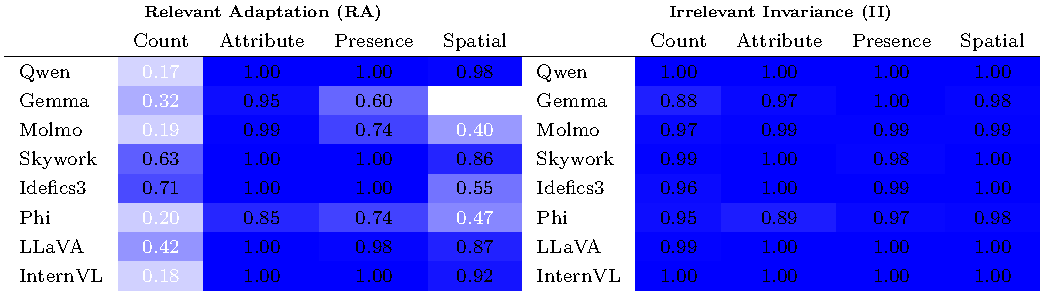
\includegraphics[width=.76\textwidth]{figures/dependency_fingerprint.pdf}
\caption{All $8\times4=32$ model--factor measurements. Relevant Adaptation
(RA) varies widely; Irrelevant Invariance (II) is predominantly high. Both are
conditional on a correct audit-base decision.}
\label{fig:behavioral_landscape}
\end{figure*}

Across all 32 cells, RA ranges from $0$ to $1$, whereas II ranges from about
$0.876$ to $1$ (Fig.~\ref{fig:behavioral_landscape}). High invariance therefore
does not imply appropriate adaptation. Qwen illustrates the distinction: it has
RA/II $=1/1$ on Attribute but RA/II $=.17/1$ on Count. It is correct on every
Count base image and follows the new preference on only $34/200$ relevant
edits. In the remaining $166/200$ cases, it retains its base prediction even
though the gold label changes, exactly the failure in
Eq.~\ref{eq:ra_retention}. Static accuracy is informative, but it does not
determine these selective response patterns.

\begin{figure*}[t]
\centering
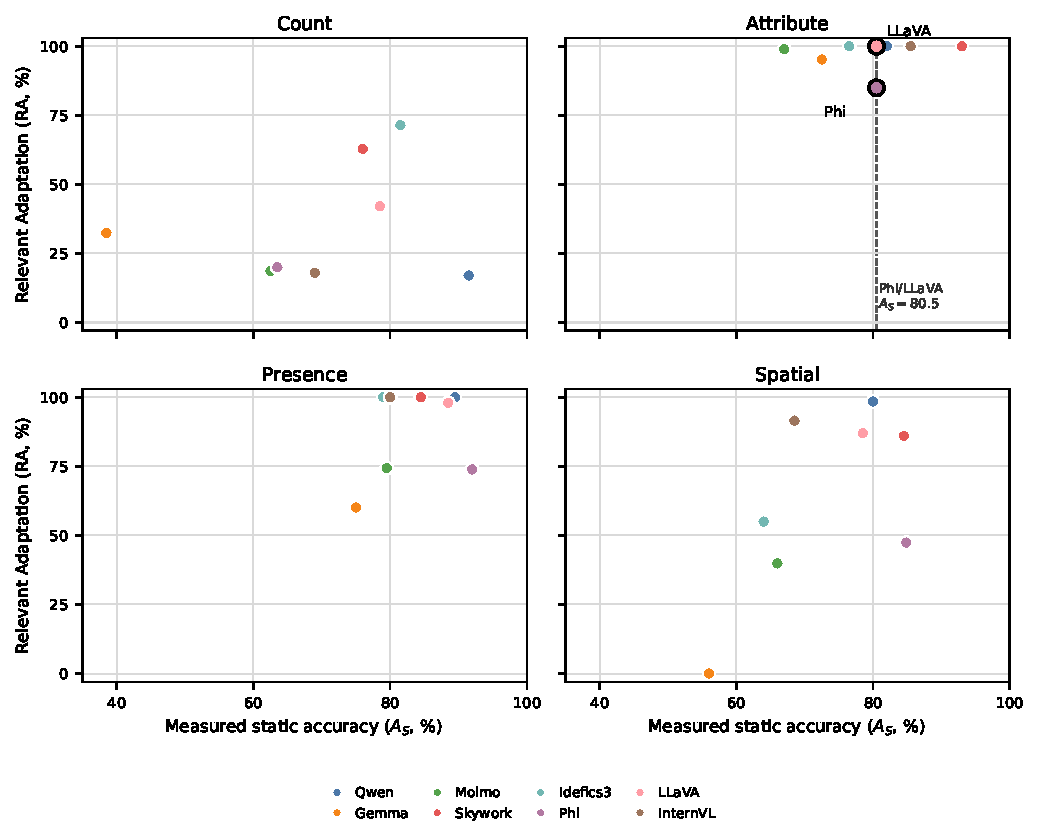
\includegraphics[width=.68\textwidth]{figures/static_vs_ra.pdf}
\caption{Measured static accuracy versus RA by factor. The Attribute panel
highlights the Phi--LLaVA exact tie at $80.5\%$ static accuracy and their
$84.95\%$ versus $100.00\%$ RA values.}
\label{fig:static_vs_ra}
\end{figure*}

\begin{figure*}[t]
\centering
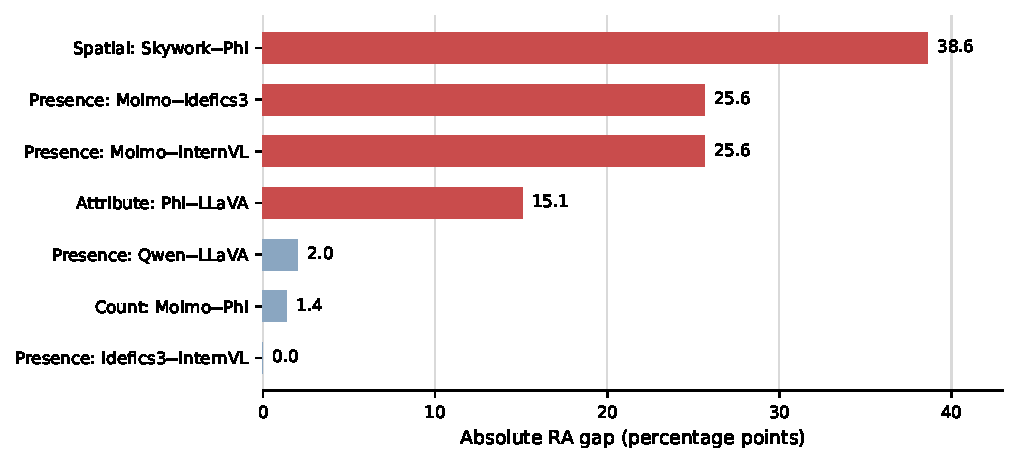
\includegraphics[width=.66\textwidth]{figures/matched_ra_gaps.pdf}
\caption{Ranked RA gaps for all seven primary matched pairs. Red bars mark
gaps of at least 10 pp.}
\label{fig:matched_pair_gaps}
\end{figure*}


\section{Robustness and Validity Checks}
\label{sec:robustness}

\subsection{Shared-Base-Correct Comparisons}

The Attribute tie is unchanged on the 186 triplets that both Phi and LLaVA
judge correctly at base: RA remains $84.95\%/100.00\%$. Across all seven
one-point matched pairs, restricting comparisons to shared base-correct support
leaves the descriptive median absolute RA gap at $15.05$ pp. This diagnostic
uses a common support for both judges; it complements rather than replaces the
judge-conditional RA definition.

\subsection{Audit-Base Accuracy}

The matched static comparison is not simply an artifact of a judge being wrong
on most audit bases. For example, on Presence, Molmo and Idefics3 have audit-base
accuracies of $99.5\%$ and $100.0\%$, respectively, but differ by $25.63$ pp in
RA. The full audit-base ledger and judge-specific conditional denominators are
reported in Table~\ref{tab:all_32_base_accuracy} in
Appendix~\ref{app:additional-results}.

\subsection{Matching-Threshold Sensitivity}

The descriptive median absolute RA gap is $15.05$ pp under the 1 pp matching
band, $15.05$ pp under the 2 pp band, and $15.14$ pp under the 3 pp band. These
bands are part of the frozen analysis plan; the complete censuses are reported
in Table~\ref{tab:threshold-sensitivity-full} in
Appendix~\ref{app:additional-results}. Pair rows share judges and
are not treated as independent observations.

\subsection{Edit-Magnitude Sensitivity and Scope}

On Attribute, relevant edits have lower average pixel-change fraction than
irrelevant edits ($0.118$ versus $0.179$). In the post-hoc Attribute subset with
matched edit magnitude, the Phi--LLaVA RA gap remains $16.8$ pp. Spatial has a
larger relevant-edit magnitude, so its $38.60$ pp Skywork--Phi gap remains
supportive rather than the headline case. The complete common-support,
paired-bootstrap, and edit-magnitude checks are reported in
Appendix~\ref{app:robustness-tables}. These checks support a limited behavioral
conclusion, not an internal-grounding claim.


\section{Conclusion}
\label{sec:conclusion}

RewardLens shows that equal or near-equal measured static accuracy can coexist
with different measured intervention behavior. The clearest case is the
$80.5\%$ Attribute tie between Phi and LLaVA, whose RA differs by $15.1$ pp;
the complete one-point census has seven pairs and a descriptive median RA gap
of $15.1$ pp. These results complement rather than invalidate static
evaluation. They apply to observable behavior on four controlled factors and
do not identify internal grounding mechanisms. Within that scope, reporting
RA and II alongside static accuracy exposes selective failures to update that a
single cross-sectional score leaves unresolved.


% --------------------------------------------------
% Statements
% --------------------------------------------------

\subsection*{AI use statement}

% TODO: Replace with final ICLR 2027-compliant disclosure.
We used generative AI tools to assist with tasks that will be disclosed
in accordance with the ICLR 2027 AI Policy for Authors.
All AI-assisted content was reviewed and verified by the authors.
The authors take responsibility for the final content of this work.

\subsection*{Reproducibility statement}

% TODO: Write after experiments and appendix are frozen.
We describe the experimental setup, evaluation protocol, and implementation
details necessary to reproduce the main results in the paper and appendix.

% --------------------------------------------------
% References
% --------------------------------------------------

\bibliography{references}
\bibliographystyle{iclr2027_conference}

% ----------下一步建议先处理 .gitignore，把这些垃圾文件隐藏/排除，然后初始化 Git，再开始正式迁移 RewardLens 正文。这样工程会干净很多。----------------------------------------
% Appendix
% --------------------------------------------------

\appendix

% !TeX root = ../main.tex
\section{Additional Results}
\label{app:additional-results}

This appendix reports the complete factor-level result ledger and the full
robustness summaries used in the main text. Percentages are reported to two
decimal places. $A_S$ is measured on the independent static set; $A_B$ is
unconditioned accuracy on the RewardLens-CLEVR base images; RA and II are
conditional on a correct base decision.

\FloatBarrier

\subsection{All Model--Factor Measurements}
\label{app:all-model-factor-results}

Table~\ref{tab:all_32_results} contains every one of the $8\times4=32$
model--factor measurements. Each factor has 200 frozen static items and 200
frozen audit triplets. All static estimates use 200 reported outcomes except
Phi-3.5-Vision on Spatial ($n=198$); no imputation is used. The conditional
denominator $n_B$ is the number of base-correct audit triplets for that model
and factor.

\begin{table*}[t]
\centering
\scriptsize
\caption{Complete model--factor ledger. Each cell is $A_S$/RA/II in percent;
the corresponding audit-base denominators are reported in
Table~\ref{tab:all_32_base_accuracy}. All $A_S$ estimates use $n=200$ except
Phi-3.5-Vision on Spatial ($n=198$; marked $^{\dagger}$); no imputation is used.}
\label{tab:all_32_results}
\setlength{\tabcolsep}{3.2pt}
\begin{tabular}{lrrrrrrrrrrrr}
\toprule
& \multicolumn{3}{c}{Count} & \multicolumn{3}{c}{Attribute}
& \multicolumn{3}{c}{Presence} & \multicolumn{3}{c}{Spatial} \\
Judge & $A_S$ & RA & II & $A_S$ & RA & II & $A_S$ & RA & II & $A_S$ & RA & II \\
\midrule
Qwen3-VL-4B & 91.50 & 17.00 & 100.00 & 82.00 & 100.00 & 100.00 & 89.50 & 100.00 & 100.00 & 80.00 & 98.50 & 100.00 \\
Gemma-3-4B & 38.50 & 32.41 & 87.59 & 72.50 & 95.19 & 97.33 & 75.00 & 60.10 & 100.00 & 56.00 & 0.00 & 97.95 \\
Molmo-7B-D & 62.50 & 18.63 & 97.06 & 67.00 & 98.96 & 98.96 & 79.50 & 74.37 & 98.99 & 66.00 & 39.86 & 99.32 \\
Skywork-VL-Reward-7B & 76.00 & 62.81 & 98.99 & 93.00 & 100.00 & 100.00 & 84.50 & 100.00 & 98.49 & 84.50 & 86.00 & 100.00 \\
Idefics3-8B & 81.50 & 71.43 & 95.77 & 76.50 & 100.00 & 100.00 & 79.00 & 100.00 & 99.50 & 64.00 & 55.00 & 100.00 \\
Phi-3.5-Vision & 63.50 & 20.00 & 95.15 & 80.50 & 84.95 & 89.25 & 92.00 & 73.89 & 97.22 & $84.85^{\dagger}$ & 47.40 & 98.44 \\
LLaVA-OneVision-7B & 78.50 & 42.08 & 98.91 & 80.50 & 100.00 & 100.00 & 88.50 & 98.00 & 100.00 & 78.50 & 87.00 & 100.00 \\
InternVL3-8B & 69.00 & 18.00 & 100.00 & 85.50 & 100.00 & 100.00 & 80.00 & 100.00 & 100.00 & 68.50 & 91.50 & 100.00 \\
\bottomrule
\end{tabular}
\end{table*}

\begin{table}[t]
\centering
\scriptsize
\caption{Complete $|\Delta A_S|\leq1$ pp matched-pair census. All gaps are
absolute percentage points.}
\label{tab:matched_pairs_1pp}
\begin{tabular}{llrrr}
\toprule
Factor & Pair & $\Delta A_S$ & $\Delta\mathrm{RA}$ & $\Delta\mathrm{II}$\\
\midrule
Spatial & Skywork--Phi & .35 & 38.60 & 1.56\\
Presence & Molmo--Idefics3 & .50 & 25.63 & .51\\
Presence & Molmo--InternVL & .50 & 25.63 & 1.01\\
Attribute & Phi--LLaVA & .00 & 15.05 & 10.75\\
Presence & Qwen--LLaVA & 1.00 & 2.00 & .00\\
Count & Molmo--Phi & 1.00 & 1.37 & 1.91\\
Presence & Idefics3--InternVL & 1.00 & .00 & .50\\
\bottomrule
\end{tabular}
\end{table}

\begin{table*}[t]
\centering
\scriptsize
\caption{Audit-base accuracy and conditional denominators for the same 32
measurements in Table~\ref{tab:all_32_results}. Each entry is $A_B$ (\%) / $n_B$.}
\label{tab:all_32_base_accuracy}
\setlength{\tabcolsep}{7pt}
\begin{tabular}{lrrrr}
\toprule
Judge & Count & Attribute & Presence & Spatial \\
\midrule
Qwen3-VL-4B & 100.0 / 200 & 100.0 / 200 & 99.5 / 199 & 100.0 / 200 \\
Gemma-3-4B & 72.5 / 145 & 93.5 / 187 & 99.0 / 198 & 73.0 / 146 \\
Molmo-7B-D & 51.0 / 102 & 96.5 / 193 & 99.5 / 199 & 74.0 / 148 \\
Skywork-VL-Reward-7B & 99.5 / 199 & 100.0 / 200 & 99.5 / 199 & 100.0 / 200 \\
Idefics3-8B & 94.5 / 189 & 100.0 / 200 & 100.0 / 200 & 100.0 / 200 \\
Phi-3.5-Vision & 82.5 / 165 & 93.0 / 186 & 90.0 / 180 & 96.0 / 192 \\
LLaVA-OneVision-7B & 91.5 / 183 & 100.0 / 200 & 100.0 / 200 & 100.0 / 200 \\
InternVL3-8B & 100.0 / 200 & 100.0 / 200 & 100.0 / 200 & 100.0 / 200 \\
\bottomrule
\end{tabular}
\end{table*}

\subsection{Full Robustness Tables}
\label{app:robustness-tables}

\paragraph{Paired bootstrap.}
For each primary matched pair, we resample matched source triplets jointly for
the two judges ($10{,}000$ replicates; seed 20270915). Table~\ref{tab:paired-bootstrap}
reports signed model-A minus model-B contrasts, so its sign depends on the
printed order. Static contrasts are resampled on shared static item identifiers;
the reported static point estimate can therefore differ slightly from the
displayed difference between separately rounded static percentages.

\begin{table*}[t]
\centering
\scriptsize
\caption{Paired-bootstrap contrasts for all primary matched pairs (percentage
points; 95\% percentile intervals). All audit contrasts resample 200 matched
source triplets jointly across the two judges.}
\label{tab:paired-bootstrap}
\setlength{\tabcolsep}{4pt}
\begin{tabular}{llrrr}
\toprule
Factor & Ordered comparison & Static $\Delta$ [95\% CI] & RA $\Delta$ [95\% CI] & II $\Delta$ [95\% CI] \\
\midrule
Spatial & Skywork $-$ Phi & $-0.51$ [$-6.06$, 5.05] & 38.60 [29.78, 47.23] & 1.56 [0.00, 3.61] \\
Attribute & Phi $-$ LLaVA & 0.00 [$-5.50$, 5.50] & $-15.05$ [$-20.43$, $-10.21$] & $-10.75$ [$-15.46$, $-6.42$] \\
Presence & Molmo $-$ Idefics3 & 0.50 [$-6.50$, 7.50] & $-25.63$ [$-31.66$, $-19.60$] & $-0.51$ [$-2.04$, 1.00] \\
Presence & Molmo $-$ InternVL & $-0.50$ [$-6.00$, 5.50] & $-25.63$ [$-31.82$, $-19.60$] & $-1.01$ [$-2.53$, 0.00] \\
Count & Molmo $-$ Phi & $-1.00$ [$-6.50$, 4.50] & $-1.37$ [$-10.23$, 7.55] & 1.91 [$-2.68$, 6.40] \\
Presence & Qwen $-$ LLaVA & 1.00 [$-3.00$, 5.00] & 2.00 [0.50, 4.00] & 0.00 [0.00, 0.00] \\
Presence & Idefics3 $-$ InternVL & $-1.00$ [$-7.00$, 5.00] & 0.00 [0.00, 0.00] & $-0.50$ [$-1.50$, 0.00] \\
\bottomrule
\end{tabular}
\end{table*}

\paragraph{Shared-base-correct support.}
Table~\ref{tab:shared-base-correct-full} recomputes RA and II on the
intersection of the two judges' base-correct sets. It is a common-support
diagnostic, not a replacement for the judge-conditional definitions in
Eqs.~\ref{eq:emp_ra}--\ref{eq:emp_ii}.

\begin{table*}[t]
\centering
\scriptsize
\caption{All seven primary matched pairs on shared base-correct support.
Entries show model-A/model-B percentages; gaps are absolute percentage points.}
\label{tab:shared-base-correct-full}
\setlength{\tabcolsep}{5pt}
\begin{tabular}{llrrrrr}
\toprule
Factor & Pair & $n_{\cap}$ & RA A/B & $|\Delta\mathrm{RA}|$ & II A/B & $|\Delta\mathrm{II}|$ \\
\midrule
Spatial & Skywork--Phi & 192 & 86.98 / 47.40 & 39.58 & 100.00 / 98.44 & 1.56 \\
Presence & Molmo--Idefics3 & 199 & 74.37 / 100.00 & 25.63 & 98.99 / 99.50 & 0.50 \\
Presence & Molmo--InternVL & 199 & 74.37 / 100.00 & 25.63 & 98.99 / 100.00 & 1.01 \\
Attribute & Phi--LLaVA & 186 & 84.95 / 100.00 & 15.05 & 89.25 / 100.00 & 10.75 \\
Count & Molmo--Phi & 100 & 17.00 / 4.00 & 13.00 & 99.00 / 100.00 & 1.00 \\
Presence & Qwen--LLaVA & 199 & 100.00 / 97.99 & 2.01 & 100.00 / 100.00 & 0.00 \\
Presence & Idefics3--InternVL & 200 & 100.00 / 100.00 & 0.00 & 99.50 / 100.00 & 0.50 \\
\bottomrule
\end{tabular}
\end{table*}

\begin{table}[t]
\centering
\scriptsize
\caption{Sensitivity to the within-factor static-matching
tolerance. All gaps are absolute percentage points.}
\label{tab:threshold-sensitivity-full}
\begin{tabular}{rrrrrr}
\toprule
Tolerance & Pairs & Median RA & 90th RA & Max RA & RA $\geq10$ pp \\
\midrule
1 pp & 7 & 15.05 & 30.82 & 38.60 & 4 \\
2 pp & 11 & 15.05 & 25.63 & 38.60 & 7 \\
3 pp & 15 & 15.14 & 34.90 & 51.64 & 11 \\
\bottomrule
\end{tabular}
\end{table}

\begin{table}[t]
\centering
\scriptsize
\caption{Image-level edit diagnostics by factor. Pixel-change fraction and
global SSIM are computed after resizing to 256 pixels; SSIM is a global RGB
statistic, not a semantic mask measurement.}
\label{tab:edit-magnitude-full}
\begin{tabular}{lrrrr}
\toprule
& \multicolumn{2}{c}{Pixel-change fraction} & \multicolumn{2}{c}{Global SSIM} \\
Factor & Relevant & Irrelevant & Relevant & Irrelevant \\
\midrule
Count & 0.229 & 0.229 & 0.925 & 0.922 \\
Attribute & 0.118 & 0.179 & 0.974 & 0.958 \\
Presence & 0.175 & 0.201 & 0.935 & 0.918 \\
Spatial & 0.375 & 0.265 & 0.817 & 0.890 \\
\bottomrule
\end{tabular}
\end{table}

As an additional post-hoc sensitivity analysis, the magnitude-matched subset
retains 459 of 800 triplets under
$\lvert p_R-p_I\rvert\leq0.05$: 191 Count, 109 Attribute, 103 Presence, and
56 Spatial triplets. On the 109 retained Attribute triplets, Phi is
base-correct on 101 and has RA $=83.17\%$; LLaVA has RA $=100.00\%$.
This is an approximately 16.8 percentage-point RA gap on that restricted
subset.

\subsection{Representative Frozen Audit Triplets}
\label{app:qualitative-triplets}

Figure~\ref{fig:representative-triplets} shows one retained PASS triplet per
factor. These are direct copies of frozen renders; no scene was regenerated or
manually edited for the manuscript. Count changes or preserves the target-color
count; Attribute recolors the target or a matched non-target; Presence removes
the queried conjunction or a matched non-target; and Spatial moves the queried
referent or a matched distractor.

\begin{figure*}[t]
\centering
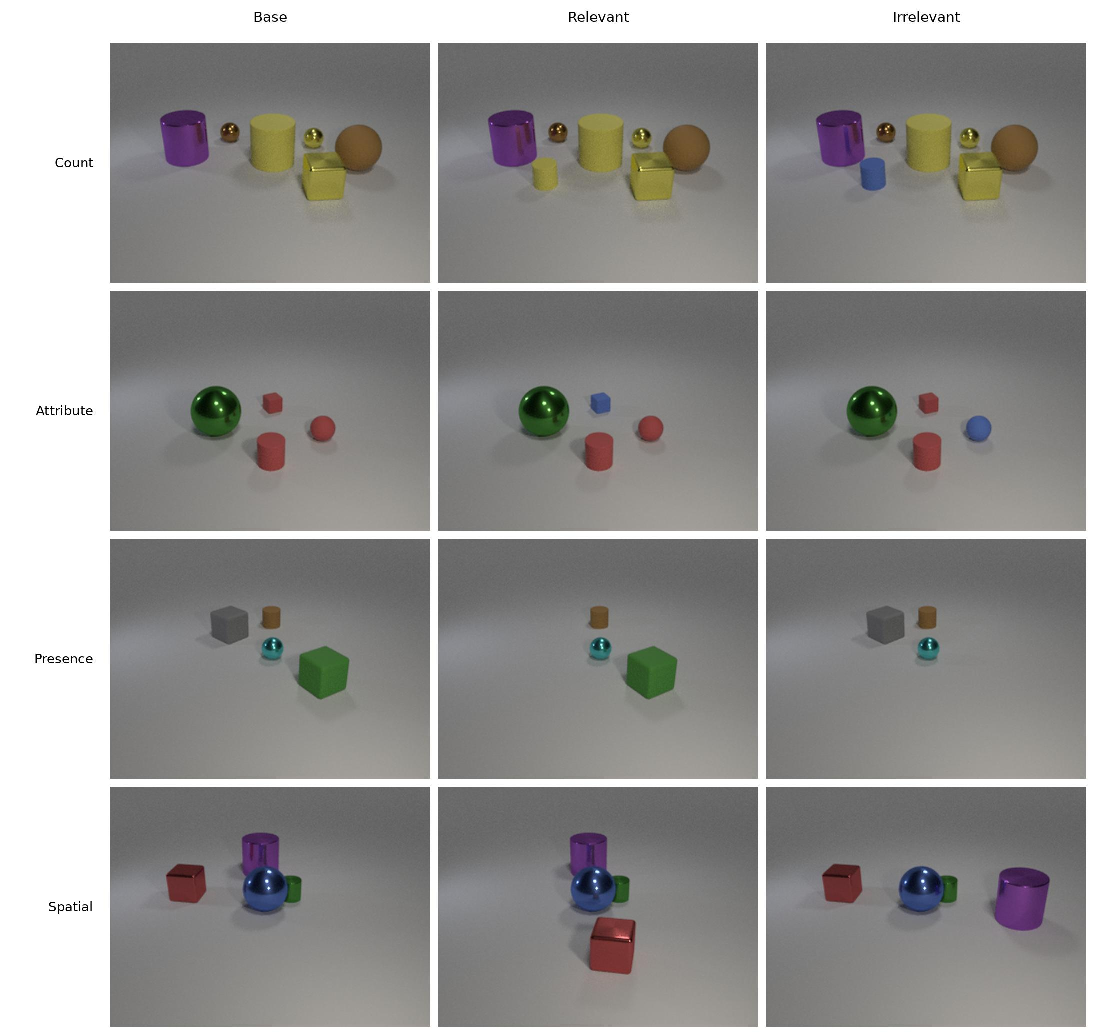
\includegraphics[width=.98\textwidth]{figures/representative_triplets.pdf}
\caption{Representative frozen RewardLens-CLEVR PASS triplets. Columns are
Base, Relevant, and Irrelevant. Rows respectively illustrate target-category
count change versus a matched non-target count change; target versus non-target
recoloring; queried-conjunction versus matched non-target removal; and queried
referent versus matched distractor translation. The source triplet identifiers
are Count \texttt{count\_000000}, Attribute \texttt{attr\_000000}, Presence
\texttt{pres\_000000}, and Spatial \texttt{spat\_000000}.}
\label{fig:representative-triplets}
\end{figure*}

% !TeX root = ../main.tex
\section{Implementation Details}
\label{app:implementation-details}


\end{document}